% Automatica autart two-column template; download provenance in template/.
\documentclass[twocolumn,nameyear]{autart}
\usepackage{fix-cm}
\usepackage[T1]{fontenc}
\usepackage{amsmath,amssymb,booktabs,graphicx}
\usepackage[authoryear,round]{natbib}
\usepackage{url}
\usepackage{needspace}
\renewcommand{\ttdefault}{lmtt}
\urlstyle{rm}
\setlength{\emergencystretch}{1em}
\raggedbottom

\begin{document}
\begin{frontmatter}
\title{Control Sensitivity and the Cost of Certifying Small Policy Improvements}
\thanks[cor1]{Corresponding author: Yeoneung Kim. Email: yeoneung@yonsei.ac.kr.}
\author[gachon]{Kyunghyun Lee}\ead{kyunghyunlee@gachon.ac.kr},
\author[yonsei]{Yeoneung Kim\thanksref{cor1}}\ead{yeoneung@yonsei.ac.kr}
\address[gachon]{Department of Computer Science, Gachon University,
1342 Seongnam-daero, Sujeong-gu, Seongnam, Gyeonggi-do 13120, Republic of Korea}
\address[yonsei]{Department of Industrial Engineering, Yonsei University,
50 Yonsei-ro, Seodaemun-gu, Seoul 03722, Republic of Korea}
\begin{keyword}
Stochastic control; Policy improvement; Incremental sensitivity;
Common random numbers; Sample complexity; Statistical certification.
\end{keyword}
\begin{abstract}
Certifying a small controller improvement can require many simulation
trajectories, even when common random numbers reduce comparison noise. We ask when
control sensitivity prevents this growth, counting the simulation needed
to certify that sensitivity. Baseline closed-loop sensitivity and an
enforced action displacement $d$ give a pathwise paired-return support
of order $d$, even for discontinuous updates. For gains proportional to
$d$, this support permits a displacement-independent validation budget;
rules uniformly valid over an unrestricted fixed ordinary range face an
$\Omega(d^{-1})$ barrier on the same favorable law. We acquire the support
from replicated Gaussian transitions with unknown noise scale. A
finite-power small-gain margin gives a uniform state envelope and an
explicit calibration budget independent of $d$, allowing transient
amplification and matrix norms above one. Every Schur-stable linear
baseline admits such a certificate. Regional sensitivity can lose the
saving through the cost of estimating escape probability. On 24
controlled plants, shared disturbances reduce comparison variance by a
mean factor of 1,796, yet ordinary-range testing makes no adoptions at
512 pairs; supplying paired support to the same test certifies all 24.
\end{abstract}

\end{frontmatter}

\section{Introduction}
A controller that already performs reasonably well may need only a
small correction. Verifying that correction can nevertheless consume
many simulation trajectories: its return gain is small, and accepting
a non-improving controller must remain unlikely. The question is whether
reliable verification must become more expensive as the permitted
correction shrinks. We study when control sensitivity prevents this
increase, after charging the simulation needed to certify the
sensitivity itself.

Our answer uses simulations in which the two controllers share initial
states and disturbances. Baseline closed-loop sensitivity can make the
range of their return difference shrink with the correction, so that
the signal and its worst-case uncertainty shrink together. A finite-power
certificate makes this information available beyond one-step contraction.
With a fixed robust margin and a gain proportional to the correction
size, acquiring the certificate and validating the gain both require
budgets independent of that size. We count both stages in the cost.

Such coupling can make the return difference much less variable than
either return separately. Common random numbers (CRN) are an
established simulation technique, also used in policy search
\citep{glasserman1992guidelines,ng2000pegasus,strens2002paired}.
Pathwise Lipschitz regularity can already imply quadratic decay of
comparison variance as a parameter change shrinks
\citep[Lemma 6.1]{glasserman1992guidelines}.

The distinction can be seen from a constant positive paired difference.
A verifier that knows only a fixed ordinary return range must still
allow a distribution with a rare large loss. Such a non-improving
distribution can produce the same positive observations until that
loss is encountered. A valid pathwise sensitivity bound can exclude the
large loss before validation starts. Thus small variance and a small
justified support provide different information. Range-dependent terms
in bounded-mean estimation are well established
\citep{mnih2008stopping,waudbysmith2024betting}; we connect their
consequences to the size of a controller correction.

Safe policy improvement provides performance guarantees for replacing
a baseline \citep{pirotta2013safe,thomas2015high}, and residual learning
constructs corrections to existing controllers
\citep{johannink2018residual}. Lipschitz decision-process analysis bounds
expected performance \citep{pirotta2015lipschitz,asadi2018lipschitz}.
Incremental stability \citep{angeli2002incremental} also informs imitation
learning sample complexity \citep{tu2022sample} and the cost of learning
robust stability certificates \citep{zhang2022adversarial}.
Our task is the post-training certification of a frozen candidate's
return gain. Baseline sensitivity bounds each paired observation,
including for a discontinuous candidate.

Data-efficient policy optimization \citep{zhao2025dataenabled} and the
connections between direct and identification-based control
\citep{dorfler2023bridging} concern controller construction.
We study information for a subsequent adoption decision and its
acquisition cost. Model-based gain certification may avoid return
validation altogether; the ordinary-range barrier concerns its stated
information class.

Statistical control analysis relates sample requirements to stability margins
\citep{gatsis2021statistical}, and closed-loop identification admits
non-asymptotic confidence constructions
\citep{szentpeteri2023nonasymptotic}. Here replicated Gaussian transitions
acquire a return envelope at a fixed matrix accuracy. Finite powers
permit transient amplification and, with a robust margin, nonlinear
residuals. Under fixed discount the pair budget is uniform in finite
horizon; transitions per pair still grow with horizon. Regional
sensitivity can lose the saving through the cost of escape information.

Section~\ref{sec:certification} states the cost comparison,
Section~\ref{sec:sensitivity} derives the control envelopes, and
Section~\ref{sec:calibration} accounts for acquisition.
Sections~\ref{sec:regional} and~\ref{sec:experiments} treat regional
sensitivity and numerical evidence. The appendices give the calibration
proofs and sequential power details.

\section{Certification and the verifier's information}\label{sec:certification}
\subsection{The adoption decision}
Fix a baseline $B$, horizon $H$ and discount $0<\gamma\le1$. Let
\[
 R(\pi)=\sum_{t=0}^{H-1}\gamma^t r(X_t,\pi_t(X_t)),
 \qquad J(\pi)=\mathbb{E}R(\pi).
\]
The candidate is frozen before validation. Each return pair shares its
initial state and disturbances; different pairs are independent.
Coupling preserves the marginal laws, so $D=R(\pi)-R(B)$ has mean
$\mu=J(\pi)-J(B)$. The verifier decides whether to adopt the candidate,
with false adoption meaning acceptance when $\mu\le0$.

The information supplied to that decision is central. If both returns
lie in a common interval of width $B_g$, then $|D|\le B_g$ follows
from the marginal ranges. A sharper \emph{paired support} $|D|\le b_d$
uses the coupling and properties of the two trajectories. A small
empirical variance or maximum does not itself justify that restriction.

For a justified half-width $b>0$, write
\begin{align*}
 \mathcal P_b&=\{P:P([-b,b])=1\},\\
 \mathcal P_b^0&=\{P\in\mathcal P_b:\mathbb{E}_PD\le0\}.
\end{align*}
An adoption rule with stopping time $\tau$ is uniformly valid at level
$\alpha$ if $\sup_{P\in\mathcal P_b^0}P(\tau<\infty)\le\alpha$.
Its power at budget $N$ is $P(\tau\le N)$ under a favorable law.
Validity alone permits always retaining the baseline; a cost comparison
therefore also specifies the probability of accepting a useful update.

\subsection{Why the ordinary range can be costly}
The range-only null class contains every law compatible with the stated
range and a nonpositive mean. Additional plant information may exclude
some of those laws. The following bound applies when the verifier must
remain valid over the full class.

\begin{prop}[Range-only adoption barrier]\label{prop:barrier}
Let an adoption rule, possibly randomized, be uniformly valid over
$\mathcal P_b^0$. If it adopts by $N$ with probability at least $1-\beta$
under $P\in\mathcal P_b$ with mean $\mu>0$, and $1-\beta>\alpha$, then
\begin{equation}\label{eq:barrier}
 N\ge\frac{\log((1-\beta)/\alpha)}{\log(1+\mu/b)}.
\end{equation}
This includes favorable laws with zero variance.
\end{prop}
\Needspace{8\baselineskip}
\begin{pf}
Set $p=b/(b+\mu)$ and $Q=pP+(1-p)\delta_{-b}$, so $\mathbb{E}_QD=0$.
Generate $Q$ observations using independent mixture indicators. With
probability $p^N$ the first $N$ observations all come from $P$; conditional
on this event their joint law, including independent internal
randomization, is the favorable one. All earlier stopping opportunities
are included. Consequently
$\alpha\ge Q(\tau\le N)\ge p^N P(\tau\le N)\ge p^N(1-\beta)$,
which yields \eqref{eq:barrier}.
\end{pf}

For the constant favorable law $P=\delta_\mu$, the null in the proof
produces $+\mu$ with probability $p=b/(b+\mu)$ and $-b$ otherwise.
Its harmful outcome has probability $\mu/(b+\mu)$, allowing positive
records of order $b/\mu$ even at zero favorable variance.
A justified variance bound below $b\mu$ could exclude this null.
The result concerns power within a budget, not every realized stopping time.

\subsection{How a shrinking support changes the cost}
Suppose instead that $|D_i|\le Cd$ and $\mu_d\ge md$ for fixed
$C,m>0$. A fixed-sample rule adopts when
\begin{equation}\label{eq:hoeffding-rule}
 \overline D_N>Cd\sqrt{2\log(1/\alpha)/N}.
\end{equation}
Hoeffding's inequality \citep{hoeffding1963probability} gives false
adoption at most $\alpha$ and power at least $1-\beta$ whenever
\begin{equation}\label{eq:validation-size}
 N\ge2(C/m)^2\bigl(\sqrt{\log(1/\alpha)}
                      +\sqrt{\log(1/\beta)}\bigr)^2.
\end{equation}
The null upper-tail allowance and the favorable lower-tail allowance
are both proportional to $Cd/\sqrt N$. Comparing their sum with the
gain $md$ cancels $d$ from the required budget. Supplying only a fixed
$B_g$ instead requires $\Omega(d^{-1})$ pairs by
Proposition~\ref{prop:barrier}, since $\mu_d\le Cd$.
The positive gain-to-displacement margin matters: support of order $d$
alone does not give constant cost for gains $o(d)$.

The numerical study uses the established sequential betting mixture
\citep{waudbysmith2024betting}
\begin{align}\label{eq:betting}
 M_n&=\sum_jw_j\prod_{i=1}^n(1+\lambda_jD_i/b),\nonumber\\
 &\hspace{1em}0\le\lambda_j\le1,\qquad\sum_jw_j=1.
\end{align}
Nonnegative weights and stakes are fixed before validation. Under the
null, $M_n$ is a nonnegative supermartingale starting at one, so adoption
at $M_n\ge1/\alpha$ is anytime-valid by Ville's inequality. An
independent calibration failure allowance is added once, and testing
levels are summed across multiple updates. A support violation triggers
fallback to the baseline. Appendix~\ref{app:sequential} gives a power
bound for a specified stake.

A paired return costs $2H$ simulator transitions; a replicated one-step
reset costs two. The acquisition analysis counts these post-training
transitions. The experiments also report totals including their fixed
training budget. Fresh validation observations are separate from those
used to fit the update.

\section{From control sensitivity to paired support}\label{sec:sensitivity}
\subsection{Why baseline sensitivity is sufficient}
Consider coupled dynamics
$X_{t+1}=f(X_t,A_t)+W_t$, with common $X_0$ and $W_t$ in both branches.
In one declared state norm let $F_B(x)=f(x,B(x))$ be
$\kappa$-Lipschitz, $f$ be $L_a$-Lipschitz in action, $B$ be
$L_B$-Lipschitz, and $r$ be separately $(L_x,L_u)$-Lipschitz.
These bounds are global for now. Require
\begin{equation}\label{eq:displacement}
 \|\pi_t(x)-B(x)\|\le d\qquad\text{for every }x,t.
\end{equation}
No continuity or derivative of $\pi_t$ is assumed.
The condition concerns the \emph{implemented} action after any safety
filter, projection or clipping; a bound on a raw learned command would
not be sufficient if its subsequent implementation violated the bound.
It also permits time-dependent feedback over the fixed evaluation horizon.

The useful decomposition evaluates the baseline at the candidate state.
It separates the candidate's local action correction from propagation
through the baseline closed loop. Comparing the candidate feedback at
two different states instead would introduce regularity of $\pi_t$
that the argument does not need.

\begin{thm}[Pathwise support]\label{thm:support}
For finite $\kappa\ge0$, set
$E_0=0$ and $E_{t+1}=\kappa E_t+L_ad$. Every coupled trajectory satisfies
$\|X_t^\pi-X_t^B\|\le E_t$, and
\begin{equation}\label{eq:general-support}
 |D|\le b_d:=\sum_{t=0}^{H-1}\gamma^t
       \bigl[(L_x+L_uL_B)E_t+L_ud\bigr].
\end{equation}
If $r(x,\pi_t(x))=r(x,B(x))=:r_B(x)$ pointwise and
$\operatorname{Lip}(r_B)\le L_{r_B}$, the sharper bound is
\begin{equation}\label{eq:equal-support}
 |D|\le b_d^{\rm eq}:=L_{r_B}\sum_{t=0}^{H-1}\gamma^t E_t.
\end{equation}
Both bounds are linear in $d$ at fixed horizon and may be intersected
with any independently justified ordinary range.
\end{thm}
\Needspace{7\baselineskip}
\begin{pf}
Write $e_t=\|X_t^\pi-X_t^B\|$. Shared noise cancels. Adding and
subtracting $f(X_t^\pi,B(X_t^\pi))$ gives
\begin{align*}
 e_{t+1}&\le\|F_B(X_t^\pi)-F_B(X_t^B)\|\\
 &\quad+L_a\|\pi_t(X_t^\pi)-B(X_t^\pi)\|\\
 &\le\kappa e_t+L_ad.
\end{align*}
Since $e_0=0$, induction gives $e_t\le E_t$. The actions on the two
branches differ by at most $d+L_BE_t$, proving
\eqref{eq:general-support}. Under the pointwise reward identity, their
stage rewards are $r_B(X_t^\pi)$ and $r_B(X_t^B)$; this proves
\eqref{eq:equal-support}.
\end{pf}

The recursion gives $E_t=L_ad\sum_{j<t}\kappa^j$, with an empty
sum at $t=0$. Thus $d$ sets the observation scale, while the coefficient
records horizon and closed-loop amplification.

The reward identity holds, for example, for
$r(x,a)=r_0(x)+c_0(x,\|a\|)$ when the update preserves the baseline
action norm at each state. It removes direct effort variation but not
the first-order effect of changed state occupation.

At fixed horizon the envelope is finite even for an expanding baseline,
although amplification may make it unhelpful. When $\kappa<1$,
$E_t=L_ad(1-\kappa^t)/(1-\kappa)$ is bounded uniformly in time.
The return bound is then uniform in horizon for fixed $\gamma<1$,
and grows at most linearly in horizon for $\gamma=1$. The finite-power
argument below obtains the same time-uniform state control when the
one-step criterion fails.
State/action-dependent disturbances require the corresponding pathwise
same-noise regularity; independent unbounded disturbances do not cancel.

\subsection{A stochastic control example with no paired noise}
\begin{cor}[A stochastic separation]\label{cor:sharp}
There is a horizon-two stochastic control family with bounded Lipschitz
rewards, displacement $d$, nonzero marginal return variance and constant
paired gain $\mu_d\asymp d$, for which ordinary-range certification needs
$\Omega(d^{-1})$ pairs while paired-support certification needs $O(1)$.
The order $d$ in Theorem~\ref{thm:support} cannot generally be reduced.
\end{cor}
\begin{pf}
Let $x_0=0$, $B=(1,0)$, $\pi=(\cos\theta,\sin\theta)$,
$f(x,a)=a_2$, $r(x,a)=\operatorname{clip}(x,-2,2)$, $H=2$ and
$\gamma=1$. Use shared $W_0\sim\operatorname{Unif}[-1,1]$ and
$\theta=2\arcsin(d/2)$, $0<d\le1/2$. Both action norms are one and
their distance is $d$. With $\kappa=0$ and $L_a=L_{r_B}=1$,
\begin{equation}\label{eq:sharp-example}
 R(B)=W_0,\quad R(\pi)=W_0+\mu_d,
 \quad \mu_d=d\sqrt{1-d^2/4}.
\end{equation}
The reward remains in its linear region on these trajectories. Each
return has variance $1/3$; independent evaluation gives contrast
variance $2/3$, whereas CRN gives $D=\mu_d$ almost surely.
The ordinary contrast bound $B_g=4$ is independent of $d$.
Theorem~\ref{thm:support} gives $b_d^{\rm eq}=d$, and
$\mu_d/d\to1$, proving sharpness. Proposition~\ref{prop:barrier}
gives the ordinary-range lower bound. A betting component with
$\lambda=1$ and weight $w>0$ crosses by
\[
 N=\left\lceil\frac{\log(1/(\alpha w))}
                          {\log(1+\mu_d/b)}\right\rceil.
\]
For $b=d$ this is bounded independently of $d$; for $b=4$ it has order
$d^{-1}$. The observations themselves are identical.
\end{pf}

The example makes the information restriction explicit. In the true
plant, one paired observation equals the exact gain, but a range-only
verifier must remain valid for the contaminating null from
Proposition~\ref{prop:barrier}. A verifier given the model-derived
support $[-d,d]$ can exclude the large harmful outcome used by that
null. The separation therefore does not contradict the elementary fact
that a \emph{known} constant positive difference establishes improvement.

\subsection{Matrix powers and actuator directions}
A scalar norm bound treats every perturbation as if it were aligned
with the most amplified direction at every step. This can be conservative
for a nonnormal baseline or an underactuated system. A finite-horizon
matrix calculation retains propagation by matrix powers and, when
available, the directions in which a correction actually enters.

Suppose $F_B(x)=Mx+h(x)$ with $\operatorname{Lip}(h)\le\ell$, and a calibration
event gives $\|M-\widehat M\|_2\le\varepsilon$. Put
$p_j=\|\widehat M^j\|_2$ and $L_\Delta=\varepsilon+\ell$.

\Needspace{16\baselineskip}
\begin{prop}[Finite-horizon envelope]\label{prop:matrix}
Set $E_0=0$ and, for $t\ge1$,
\begin{equation}\label{eq:matrix}
 E_t=L_ad\sum_{j=0}^{t-1}p_j+
       L_\Delta\sum_{s=0}^{t-1}p_{t-1-s}E_s.
\end{equation}
The state and reward bounds of Theorem~\ref{thm:support} hold with this
envelope, without requiring $\|\widehat M\|_2<1$.
If $f(x,a)-f(x,B(x))=G_0v(x,a)$ for known $G_0$ and
$\|v(x,a)\|\le\|a-B(x)\|$, replace the first term by
$d\sum_{j<t}\|\widehat M^jG_0\|_2$.
\end{prop}
\begin{pf}
Let $z_t=X_t^\pi-X_t^B$,
$h_\Delta(x)=(M-\widehat M)x+h(x)$ and
$v_t=f(X_t^\pi,\pi_t(X_t^\pi))-f(X_t^\pi,B(X_t^\pi))$.
Then $z_0=0$, $\operatorname{Lip}(h_\Delta)\le L_\Delta$ and
\[
 z_t=\sum_{s=0}^{t-1}\widehat M^{t-1-s}
       [h_\Delta(X_s^\pi)-h_\Delta(X_s^B)+v_s].
\]
Take norms and use induction for \eqref{eq:matrix}. If $v_s=G_0u_s$
with $\|u_s\|\le d$, retain $\widehat M^{t-1-s}G_0$ in the forcing
term. The stage-reward argument is unchanged. All coefficients are
independent of $d$, so the recursion remains linear in $d$.
\end{pf}
The input refinement uses the same matrix-confidence event. For a target
actuator $G_0T$ with unknown $\|T\|_2\le1$, its assumption holds by
taking $u_s=T[\pi_s(X_s^\pi)-B(X_s^\pi)]$. It can improve an
underactuated envelope because transiently amplified directions need not
be directly actuated.

\subsection{A uniform envelope from finite powers}\label{sec:blocks}
A matrix can amplify a perturbation initially and still contract after
several steps. A useful block must leave enough of that contraction to
absorb matrix uncertainty and the nonlinear residual. For a fixed search
cap $K$, define
\begin{align}\label{eq:block-margin}
 \widehat S_k&=\sum_{j=0}^{k-1}p_j,\qquad
 \widehat\eta_k=1-p_k-L_\Delta\widehat S_k,\nonumber\\
 \widehat\Gamma&=\min_{1\le k\le K:\widehat\eta_k>0}
                   \widehat S_k/\widehat\eta_k.
\end{align}
An empty minimum means that no certificate is available. The ratio
balances amplification within a block against the remaining contraction
margin. The proof uses geometric series and the classical small-gain
argument \citep{doyle1992feedback}. The resulting return support can
be certified from data, as developed in Section~\ref{sec:calibration}.

\begin{cor}[Uniform envelope]\label{cor:blocks}
On the event in Proposition~\ref{prop:matrix}, a
finite $\widehat\Gamma$ gives, for all $t\ge0$,
\begin{equation}\label{eq:uniform-state}
 \|X_t^\pi-X_t^B\|\le L_ad\widehat\Gamma.
\end{equation}
Writing $H_\gamma=\sum_{t=0}^{H-1}\gamma^t$, a valid support is
\begin{equation}\label{eq:block-support}
 b_H=dH_\gamma[L_u+(L_x+L_uL_B)L_a\widehat\Gamma].
\end{equation}
Under the pointwise reward identity use
\[
 b_H=dH_\gamma L_{r_B}L_a\widehat\Gamma.
\]
For known actuator image $G_0$, the numerator $L_a\widehat S_k$
in the state bound may be replaced by
$\sum_{j<k}\|\widehat M^jG_0\|_2$.
\end{cor}
\begin{pf}
For a feasible $k$, $p_k<1$ and grouping powers into blocks gives
\[
 \sum_{j\ge0}p_j\le\widehat S_k/(1-p_k).
\]
For finite $T$, set $V_T=\max_{t\le T}\|X_t^\pi-X_t^B\|$.
Proposition~\ref{prop:matrix} yields
\[
 V_T\le\frac{\widehat S_k}{1-p_k}(L_ad+L_\Delta V_T).
\]
Rearranging and minimizing over feasible blocks proves
\eqref{eq:uniform-state}; the reward bounds follow as before.
Grouping the actuator products in the same way gives the refined
numerator, with the same denominator $\widehat\eta_k$.
\end{pf}

All block lengths use one matrix-confidence event, so minimizing the
bound needs no extra failure allocation. The certificate is reusable
across horizons and displacements; separate adoption decisions need
their testing allocations. For $\gamma<1$, $H_\gamma\le(1-\gamma)^{-1}$
gives a horizon-uniform coefficient. At fixed horizon, linearity in $d$
already follows from Proposition~\ref{prop:matrix} without stability.

\section{Acquiring the envelope and accounting for cost}\label{sec:calibration}
The control envelope changes the return-validation cost only if it can
be justified at an acceptable cost of its own. We give a concrete
calibration scheme using a simulator that can reset to chosen states.
At each reset it produces two baseline transitions with independent
noise. Their difference estimates noise scale; their average estimates
the baseline response. These calibration replicates are separate from
the common-noise trajectory pairs used for validation.

\subsection{Certifying baseline sensitivity}
Assume $F_B(x)=Mx+h(x)$, $h(0)=0$ and a known global
$\operatorname{Lip}(h)\le\ell$. At independent reset states
$x_i\in\mathbb{R}^n$, observe
\[
 y_{ij}=F_B(x_i)+w_{ij},\qquad j=1,2,
\]
where the noises are independent $N(0,\sigma^2I_n)$. Let $X$ have
rows $x_i^\top$, $Y_j$ have rows $y_{ij}^\top$, and let
$G=X^\top X$ be nonsingular. Compute
\[
 \widehat M^\top=G^{-1}X^\top(Y_1+Y_2)/2,
 \qquad s^2=\frac{\|Y_1-Y_2\|_F^2}{2nN}.
\]
The replicate difference cancels the unknown response, including the
nonlinear residual. Gaussianity makes this difference independent of
the replicate mean. It therefore supplies the noise estimate needed to
calibrate regression uncertainty. Neither $M,h$ nor $\sigma$ is supplied
to the estimator. Write $F_{a,b;u}$ for the $u$-quantile of an
$F$ distribution.

\begin{prop}[Baseline calibration]\label{prop:calibration}
Define the matrix-error radius
\begin{align}\label{eq:matrix-radius}
 \widehat\varepsilon={}&
 \frac{s\sqrt{n^2F_{n^2,nN;1-\delta}}}
      {\sqrt{2\lambda_{\min}(G)}}\nonumber\\
 &+\ell\sqrt{\operatorname{Tr}(G)/\lambda_{\min}(G)}.
\end{align}
With probability at least $1-\delta$,
$\|\widehat M-M\|_2\le\widehat\varepsilon$. Consequently
\begin{equation}\label{eq:kappa-hat}
 \widehat\kappa=\|\widehat M\|_2+\widehat\varepsilon+\ell
\end{equation}
bounds global baseline sensitivity. Either this scalar bound or the
finite-power certificate with $L_\Delta=\widehat\varepsilon+\ell$
can supply support. Fresh validation at level $\alpha$ gives
unconditional false adoption at most $\alpha+\delta$.
\end{prop}

The certificate accounts separately for regression noise, residual bias
and the residual's own sensitivity. Appendix~\ref{app:pivot} derives
the exact pivot. The residual bound and the action and reward constants
remain model assumptions; finite reset data do not establish global
regularity. Reset states must also excite every state direction, as
expressed by nonsingularity of $G$.

One freezes the update, calibrates the baseline and tests fresh paired
returns. Without a useful certificate, retain the baseline or use a
separately justified envelope. Support calibration leaves the sign of
the gain to return validation.

\subsection{Total cost without one-step contraction}
A smaller correction could be costly if it required a progressively
more accurate matrix estimate. A fixed positive robust margin avoids
this: one fixed accuracy suffices. The next theorem quantifies the
acquisition and validation budgets. Fix a block cap $K$ and target matrix accuracy
$e_*>2\ell\sqrt n$. For $a_j=\|M^j\|_2$, define deterministic
perturbation bounds
\begin{align}\label{eq:q-powers}
 q_0&=1,\qquad
 q_j=a_j+e_*\sum_{s=0}^{j-1}a_{j-1-s}q_s,\nonumber\\
 S_*&=\sum_{j=0}^{K-1}q_j,\qquad
 \eta_*=1-q_K-(\ell+e_*)S_*.
\end{align}
These are analysis constants; the verifier uses only
$(\widehat M,\widehat\varepsilon)$ in \eqref{eq:block-margin}.
A positive $\eta_*$ guarantees that the block certificate remains useful
when both matrix error and its reported radius are at most $e_*$.

\begin{thm}[Total cost]\label{thm:cost}
Assume Gaussian resets $N(0,\sigma_x^2I_n)$ and $\sigma_x,\sigma>0$.
Fix an integer $K\ge1$ and $e_*>2\ell\sqrt n$ with $\eta_*>0$ in
\eqref{eq:q-powers}. Let $\alpha,\beta,\delta\in(0,1/2)$.
Choose $N_c$ by \eqref{eq:ncal}, calibrate the matrix radius at
level $\delta/4$, and search blocks $1,\ldots,K$ as in
\eqref{eq:block-margin}. Retain $B$ if none is certified.
For a frozen update satisfying \eqref{eq:displacement} and
$\mu_d\ge md$ with fixed $m>0$, put
\begin{equation}\label{eq:cost-C}
 C_H=H_\gamma[L_u+(L_x+L_uL_B)L_aS_*/\eta_*].
\end{equation}
Under the pointwise reward identity use
\[
 C_H=H_\gamma L_{r_B}L_aS_*/\eta_*.
\]
Let $N_v$ be the ceiling of \eqref{eq:validation-size} with $C=C_H$.
Apply \eqref{eq:hoeffding-rule} with $Cd$ replaced by the calibrated
$b_H$ from \eqref{eq:block-support}.
False adoption is at most $\alpha+\delta/4$, power is at least
$1-\beta-\delta$, and the transition cost is at most
\begin{equation}\label{eq:total-cost}
 2N_c+2HN_v,
\end{equation}
with $N_c,N_v$ independent of $d$. When $\gamma<1$, replacing
$H_\gamma$ by $(1-\gamma)^{-1}$ makes $N_v$ uniform over finite
horizons with the same gain margin. For the same favorable law, any
ordinary-range rule with power $1-\beta$ obeys
\begin{equation}\label{eq:cost-lower}
 N\ge\frac{B_g}{C_Hd}\log\frac{1-\beta}{\alpha}.
\end{equation}
\end{thm}

\medskip\noindent\textbf{Why acquisition remains finite.}
The explicit allocation in Appendix~\ref{app:cost} ensures, with
probability at least $1-\delta$, that
$\|\widehat M-M\|_2\le\widehat\varepsilon\le e_*$.
The perturbation recursion then bounds each $p_j$ by $q_j$, so
$\widehat\eta_K\ge\eta_*$ and $\widehat\Gamma\le S_*/\eta_*$.
Corollary~\ref{cor:blocks} supplies a support no larger than $C_Hd$.
The matrix accuracy target is fixed as $d$ shrinks, while support and
gain shrink together in validation. The proof and constants are in
Appendix~\ref{app:cost}.

\Needspace{9\baselineskip}
For a linear baseline ($\ell=0$), every Schur-stable $M$ has a finite
$K$ with $a_K<1$. Continuity of \eqref{eq:q-powers} at $e_*=0$
then gives a positive admissible target, even if $\|M\|_2>1$.
For nonlinear residuals, the stated robust margin must still hold.
Transient growth now affects the required accuracy and the coefficient
$S_*/\eta_*$ instead of being excluded by one-step contraction.

The allocation assumes bounds on noise, matrix geometry and the gain
margin; it is a sufficient budget, not an adaptive sample-selection
guarantee. For matched overall
power, replace $\beta$ by $\beta+\delta$ in the ordinary-range comparison.
The sequential bound in Appendix~\ref{app:sequential} applies with
$C=C_H$. An unknown Gaussian covariance can provide the same block
gate through Appendix~\ref{app:covariance}; the explicit allocation here
is for isotropic noise.

\subsection{A baseline that expands in one step}\label{sec:nonnormal}
Consider
\begin{align}\label{eq:nonnormal-example}
 M&=\begin{pmatrix}1/2&1\\0&1/2\end{pmatrix},\nonumber\\
 f(x,a)&=Mx+.001\tanh(x)+(0,a)^\top.
\end{align}
Use $B=0$, $\pi_d=d$, $X_0=0$, shared i.i.d. disturbances
$N(0,.005^2I_2)$ and reward $r(x,a)=\tanh(x_1)$.
Here $\rho(M)=.5$ but $\|M\|_2=1.2071$, so the Euclidean
one-step criterion fails. With $K=4$, $e_*=.02$, $\ell=.001$,
\eqref{eq:q-powers} gives $S_*=4.1781$ and $\eta_*=.3196$.
For $\delta=.05$ and $\sigma_x=1$, \eqref{eq:ncal} requires
$N_c=173$ replicated resets, or 346 calibration transitions.
For $0<d\le.1$ and $H\ge3$, the gain has a uniform positive
linear lower bound at any fixed $0<\gamma<1$; the short proof is in
Appendix~\ref{app:example}. Thus the acquisition and pair-budget
conclusions apply to an actual stochastic control family outside
one-step contraction. This is an analytic example, separate from the
frozen numerical study below.

\section{Regional support: the price of escape information}\label{sec:regional}
The global acquisition result raises a natural qualification: can one
obtain the same saving when regularity is known only in a region visited
by the baseline? A trajectory tube transfers that regularity to the
candidate while the baseline stays in the region. Outside it, the
ordinary range must still be charged. The resulting correction depends
on escape probability, not only on the local sensitivity coefficient.

Global sensitivity is sufficient but can be unrealistic. Fix a closed
region $K$, baseline, environment, initial-state law and horizon before
escape calibration. In the same norm let
$K_\rho=\{x:\operatorname{dist}(x,K)\le\rho\}$ and assume the
sensitivity and reward bounds of Theorem~\ref{thm:support} only on
$K_\rho$. Require $\rho\ge\max_{t\le H}E_t$ and a global return
bound $|D|\le B_g$, including trajectories that escape. Define
$\mathcal A=\{X_t^B\in K,\ 0\le t\le H\}$ and
$p_e=P(\mathcal A^c)$.

\begin{prop}[Corrected regional adoption]\label{prop:regional}
Let $b=\min(B_g,b_d)>0$ (or use $b_d^{\rm eq}$) and
$Y=\operatorname{clip}(D,-b,b)$. An upper confidence bound
$\bar p_e$ from independent baseline rollouts with error $\delta_e$
gives the allowance $q=(B_g-b)\bar p_e$. Conditional on its coverage,
\begin{equation}\label{eq:escape-bias}
 |\mathbb{E} Y-\mu|\le q.
\end{equation}
Betting with factors $1+\lambda_i(Y_i-q)/(b+q)$, for predictable
$0\le\lambda_i\le1$, controls false adoption by
$\alpha+\delta_e$ at threshold $1/\alpha$. Independently calibrated
regional sensitivity adds its own failure probability.
\end{prop}
\begin{pf}
On $\mathcal A$, the one-step induction in Theorem~\ref{thm:support}
keeps the repaired state within $K_\rho$, so $|D|\le b$ and $Y=D$.
Everywhere $|Y-D|\le B_g-b$, yielding \eqref{eq:escape-bias}.
Under $\mu\le0$, $\mathbb{E}(Y-q)\le0$ and $(Y-q)/(b+q)\in[-1,1]$.
The nonnegative supermartingale argument proves the claim; add the
escape-calibration failure probability.
\end{pf}

Clipping can reduce the gain by $q$, and correcting the null costs another
$q$: $\mathbb{E} Y-q\ge\mu-2q$. If $\mu>2q$, a fixed-sample test
$\overline Y_N>q+b\sqrt{2\log(1/\alpha)/N}$ has conditional
power at least $1-\beta$ for
\begin{equation}\label{eq:regional-N}
 N\ge\frac{2b^2}{(\mu-2q)^2}
     \bigl(\sqrt{\log(1/\alpha)}+\sqrt{\log(1/\beta)}\bigr)^2.
\end{equation}
Thus $b=O(d)$, $\mu\ge md$ and $q\le\eta md$, $0<\eta<1/2$,
preserve constant validation cost. The remaining question is how much
simulation is needed to make $q$ this small.

With zero escapes in $N_e$ independent episodes, the one-sided exact
binomial endpoint \citep{clopper1934use} is
\[
 \bar p_e=1-\delta_e^{1/N_e}\le\log(1/\delta_e)/N_e.
\]
A sufficient zero-escape-record allocation is
$N_e\ge(B_g-b)\log(1/\delta_e)/(\eta md)$, of order $d^{-1}$
for fixed $B_g$. For this endpoint that order is also required as
$d\downarrow0$, since $1-e^{-a/N_e}\sim a/N_e$.
This cost concerns the stated endpoint on a zero-escape record.
Structural information about escape can change it, just as return
structure changes the ordinary-range barrier.
Each escape episode costs $H$ transitions. Analytic invariance instead
sets $p_e=q=0$ without sampling. A zero observed escape count does not
establish invariance, and fixed positive escape probability can dominate
arbitrarily small gains even when it is known exactly.

\section{Numerical evidence on frozen controller updates}\label{sec:experiments}
The experiments hold each learned controller fixed and change the noise
coupling or support information supplied to its verifier. This separates
variance reduction from the saving due to a justified support bound.
Training, calibration, certification and independent performance
evaluation use separate stages. Plant seeds are the statistical units;
means include censored and futility stops. All results below use the
previously frozen policies, records and allocations.

\begin{figure*}[t]
\centering
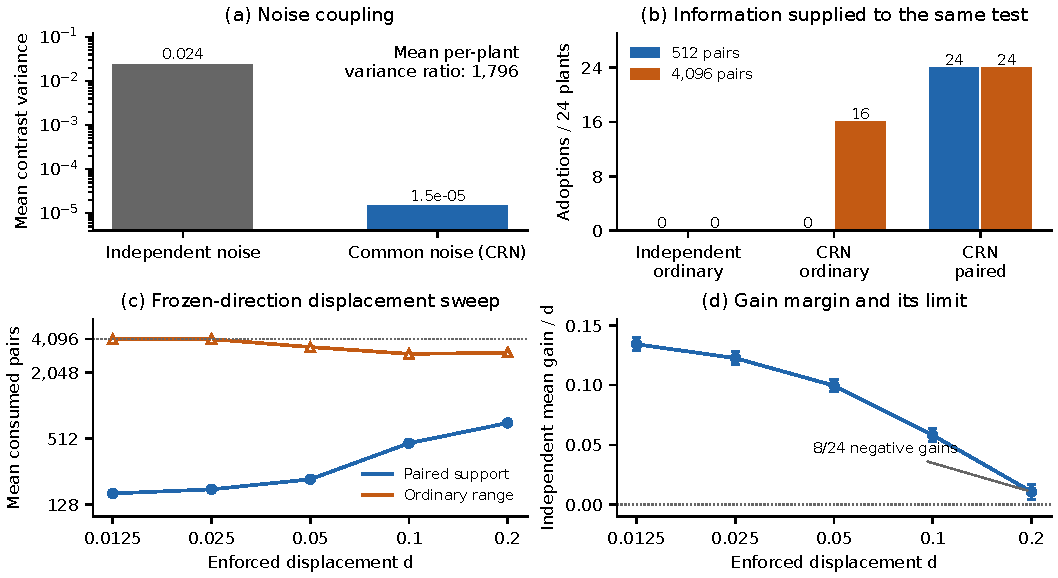
\includegraphics[width=\textwidth]{certification_mechanism.pdf}
\caption{The same 24 controlled plants. (a) Independent-noise and CRN
contrast variances; the mean per-plant ratio is 1,796.
(b) Adoptions under ordinary range and paired support.
(c) Mean pairs in the fresh-noise displacement sweep, including futility
and censoring at 4,096 (open markers).
(d) Independently evaluated gain/displacement, with across-plant SE.
Directions are rescaled without retraining; panels are related comparisons.}
\label{fig:mechanism}
\end{figure*}

\subsection{Controlled stochastic plants and protocol}
There are 24 plants in dimensions $n=4,8,16$, eight seeds per dimension.
Let $O,C,U$ be orthogonal and $S$ skew-symmetric with $\|S\|_2=1$.
Set $A=.95I+.005S$, $G_0=.1O$, $K=-.5O^\top$, and target actuator
$G_a=G_0\exp(T)\operatorname{diag}(e)$, where $T$ is skew-symmetric,
$\|T\|_2=.35$ and $e_j\in[.8,1]$. With $Q=U\operatorname{diag}(q)U^\top$
and logarithmically spaced $q_j\in[.25,2]$, use
\begin{align}\label{eq:plant}
 X_{t+1}&=AX_t+G_aA_t+.005\tanh(CX_t)+.035Z_t,\nonumber\\
 B(x)&=Kx,\nonumber\\
 r(x,a)&=-.05[1-e^{-x^\top Qx}+.1(1-e^{-\|a\|^2})].
\end{align}
Here $Z_t\sim N(0,I)$, $X_0\sim N(0,.25I)$, $H=40$ and
$\gamma=e^{-.01}$. Rewards are globally bounded despite unbounded states.
The public uncertainty set gives
\begin{align*}
 \kappa&=\|A+G_0K\|_2+\tfrac12\Delta_G+.005<1,\\
 \Delta_G&=.1[2\sin(.35/2)+.2].
\end{align*}
Also $L_a=.1$, $L_B=.5$, $L_x=.05\sqrt{4/e}$,
$L_u=.005\sqrt{2/e}$ and $L_{r_B}\le L_x+L_uL_B$.
The ordinary half-width is $B_g=.055\sum_{t<40}\gamma^t$.



A ridge learner scores rotations of $B(x)$ using paired-return queries,
preserves the baseline action norm and enforces $d=.05$.
It receives no target matrices or simulator derivatives and retains
the unchanged action when no score is positive. Query branches share
noise and follow the baseline after the queried action. Anchor and
query trajectories together cost 81,920 training transitions.
The artifact specifies features, rotation limits, ridge penalty,
query allocations and seeds. The resulting policy can be discontinuous.

All fixed-policy comparisons use the following validation protocol.
The fixed mixture \eqref{eq:betting} has stakes
$1,1/2,\ldots,1/128$ and weights $1/2,1/14,\ldots,1/14$.
Inspect every 16 pairs and at the cap; a separate negative-tail test can
stop for futility. Each pair costs 80 transitions. The ordinary and
paired-support tests receive the same ordered differences, except in the
explicit independent-noise ablation. Independent evaluation uses 4,096
pairs. Known-support comparisons retain
$\alpha=.05/(24\cdot2\cdot3\cdot2\cdot2)$; calibrated comparisons
retain $\delta_c=.025/(24\cdot3)$ and
$\alpha=.025/(24\cdot3\cdot2\cdot3\cdot2\cdot2)$.
These are the original family allocations, not retuned levels.



\subsection{Variance, support and charged calibration}
At $d=.05$, CRN reduces contrast variance by a mean per-plant factor of
1,796 (range 933--2,774). Neither independent nor CRN evaluation with
ordinary range adopts at 512 pairs. With CRN and paired support the same
fixed mixture adopts all 24 (Fig.~\ref{fig:mechanism}). At 4,096 pairs,
CRN/ordinary range adopts 16/24 versus zero with independent noise;
variance reduction helps, but does not explain the primary-budget saving.

\begin{table}[t]
\centering\small
\begin{tabular}{@{}lrrr@{}}
\toprule
Information & Adopt & Deployed gain & Transitions\\
 & & $(\times10^3)$ & used\\
\midrule
Known support & 24/24 & $4.995\pm.255$ & 99,947\\
Ordinary range & 0/24 & $0$ & 122,880\\
Calibrated support & 22/24 & $4.729\pm.375$ & 110,496\\
Ordinary (+pairs) & 0/24 & $0$ & 126,960\\
\bottomrule
\end{tabular}
\caption{Primary frozen-policy comparisons. Deployed gain is measured
on the independent evaluation bank; $\pm$ is across-plant SE.
Mean transitions used include training, calibration and validation until
stopping. Known-support arms allow 512 pairs. Calibration costs 4,096
transitions and retains 512 pairs; its ordinary comparator instead
receives 563 pairs. Allocated totals are 122,880 and 126,976; the latter
ordinary arm leaves 16 transitions unused.}
\label{tab:primary}
\end{table}

With known residual limit $\ell=.005$, 2,048 replicated resets cost
4,096 transitions. Charging this acquisition cost still permits 22/24
adoptions versus 0/24 when the ordinary comparator spends the same
allowance on extra pairs (Table~\ref{tab:primary}). Known-support and
calibrated comparisons reuse policies and return banks; their outcomes
are not independent replications.
Rescaling the 24 frozen directions from $d=.05$ to $.0125$ preserves
positive independently estimated gains and mean gain/$d$ of about
$.100$--$.134$. Supported betting uses 162--218 mean pairs and adopts
all updates. Both smallest-displacement ordinary-range conditions are
censored at 4,096, so the experiment does not estimate their asymptotic
$d^{-1}$ rate. At $d=.2$, mean gain/$d$ falls to $.011$; eight estimated
gains become negative, and supported betting retains the baseline on
those eight. The gain-margin condition cannot be extrapolated to large
updates.

\subsection{An underactuated mechanical example}
The scalar plants establish the coupling and support mechanism. We next
ask whether retaining known actuator directions makes a practical
difference when matrix propagation is used. This comparison changes the
envelope while keeping the matrix-confidence event, learned update and
return observations fixed.
On 16 separately frozen underactuated spring--mass plants, retaining
$\widehat M^jG_0$ in Proposition~\ref{prop:matrix} permits 16/16 primary
adoptions, versus none for either the unrefined matrix envelope or ordinary
range. For $p=4,8$ positions and $p$ velocities, the nominal Euler matrices are
\[
 A_0=\begin{pmatrix}I&.05I\\-.05S_m&I-.05D_m\end{pmatrix},
 \quad G_0=\begin{pmatrix}0\\.05E\end{pmatrix}.
\]
Here $S_m=\operatorname{diag}(s)+.25L^\top L$, $s_j\in[.8,1.2]$,
$L=I-I_{+1}$, $D_m$ has diagonal entries in $[.35,.45]$, and $E$
selects alternating force inputs. Nominal LQR weights
$Q_m=\operatorname{diag}(2I,.3I)$ and $R_m=.5I$ define the baseline.
The target uses $.85D_m$, an actuator rotation of spectral angle $.35$,
efficiencies in $[.8,1]$, and velocity residual $-.001\tanh(q)$.
The residual limit is $.001$, displacement is $.15$, and the reward uses
$Q_m$ in \eqref{eq:plant} with effort weight $.02$. Reset covariance is
$.09I$, and the unknown disturbance covariance has rotated eigenvalues
between $.5(.015)^2$ and $2(.015)^2$.

There are $p/2$ force inputs, so corrections enter only selected
velocity coordinates. The position--velocity coupling then spreads
their influence through the baseline dynamics. The products
$\widehat M^jG_0$ retain this route of entry; replacing them by
$\|\widehat M^j\|_2\|G_0\|_2$ also allows forcing in directions the
actuator cannot reach in one step.
Calibration uses 8,192 replicated
resets and the rowwise covariance pivot \eqref{eq:rowwise}; supported
tests have 512 pairs and the equal-cost ordinary arm has 716.
At an extended common cap of 4,096, all three tests succeed, with mean
counts 295, 587 and 2,582 respectively. Table~\ref{tab:mechanical} separates the primary budget from the
extended common budget. The unrefined envelope eventually succeeds too;
the observed benefit is that the actuator-aware bound makes the same
calibrated information useful with fewer return pairs.

\begin{table}[t]
\centering
\begin{tabular}{@{}lrr@{}}
\toprule
Envelope & Primary & Extended mean\\
 & adoptions & pairs\\
\midrule
Actuator-aware matrix & 16/16 & 295\\
Unrefined matrix & 0/16 & 587\\
Ordinary range & 0/16 & 2,582\\
\bottomrule
\end{tabular}
\caption{The same 16 frozen mechanical updates. Supported primary
tests allow 512 pairs; the ordinary comparator allows 716 after its
calibration saving is converted to return pairs. Extended tests all
allow 4,096 pairs and all adopt 16/16. Counts are rounded means.}
\label{tab:mechanical}
\end{table}

The frozen dynamics, policies, banks and allocations are included in the artifact. This experiment
illustrates how actuator geometry can make a calibrated support useful
at a limited validation budget.

\subsection{Finite-power acquisition and a model-based reference}\label{sec:block-study}
We additionally test \eqref{eq:nonnormal-example} at $H=3$ and
$\gamma=.95$, with 24 independent calibration/validation replications.
Each uses 173 replicated resets: no one-step contraction gate passes,
but all certify block length four. Methods share banks and the known
actuator image. Each decision has error allowance $.05$:
matrix coverage uses $.0125$ and calibrated return testing uses $.0375$.
The ordinary test uses $.05$ and $B_g=2(\gamma+\gamma^2)$, since
the initial reward is zero. Tests use \eqref{eq:betting}, inspected every
16 pairs, with caps 2,048 (supported) and 2,105 (ordinary, spending its
calibration saving). Displacements reuse noises. Zero and negative
controls produce no adoptions.

\begin{table}[t]
\centering\small
\begin{tabular}{@{}lrrrr@{}}
\toprule
$d$ & Ordinary & Finite-$H$ & Block & Model\\
\midrule
$.05$ & 1,824 & 442 & 1,018 & 346\\
$.025$ & 3,648 & 442 & 1,018 & 346\\
$.0125$ & 7,200 & 442 & 1,018 & 346\\
\bottomrule
\end{tabular}
\caption{Mean transitions consumed until decision; all methods
adopt 24/24 positive updates. Informed methods include 346 calibration
transitions. Finite-$H$: Proposition~\ref{prop:matrix}; Block:
Corollary~\ref{cor:blocks}; Model: Appendix~\ref{app:model-reference},
using the same calibration data without return validation.}
\label{tab:block-study}
\end{table}

Block validation uses 112 pairs at each displacement, versus 16 for
the tighter finite-horizon envelope. The model bound is already positive
from calibration: control information can support direct gain
certification too. The block bound is uniform in time; the model check
exploits the special horizon-three structure.

\section{Scope of the certification claim}
The gain margin $\mu_d\ge md$ is a condition for verification power,
not a guarantee from learning. The block theorem needs a positive
robust margin. Section~\ref{sec:block-study} checks its calibrated
support with sequential testing; it does not assess tightness of the
fixed-sample sufficient allocation in Theorem~\ref{thm:cost}.

Residual, action and reward regularity remain model assumptions.
Replicated transitions certify matrix uncertainty, not global regularity.
Regional information requires the escape correction in
Section~\ref{sec:regional} or a valid invariance argument.
Expected-return improvement does not establish state-constraint safety
or transfer automatically to a different physical plant.

\section{Conclusion}
Baseline sensitivity links controller displacement to paired-return
support. For proportional gains and a fixed robust margin, finite-power
calibration and validation have displacement-independent budgets,
including transiently expanding baselines. Under fixed discount the pair
budget is uniform in finite horizon. Regional escape information can
restore inverse-displacement cost. The resulting design question is
which information suffices for a reliable adoption decision and whether
its acquisition costs less than the validation it saves.

\section*{Funding}
Yeoneung Kim is supported by National Research Foundation of Korea (NRF)
grants funded by the Korea government (MSIT)
[RS-2023-00219980 and RS-2026-25490291], and by Yonsei University.
\section*{Declaration of competing interest}
The authors declare no competing interests.
\section*{CRediT authorship contribution statement}
\textbf{Kyunghyun Lee:} Methodology, software, investigation, validation,
visualization, writing---original draft, writing---review and editing.
\textbf{Yeoneung Kim:} Conceptualization, methodology, formal analysis,
supervision, writing---original draft, writing---review and editing.
\section*{Data availability}
Frozen experiment code and records are available at
\url{https://github.com/yeoneung/crn_policy}. The additional finite-power
study code and records accompany the submission package.
The manuscript uses synthetic data only.
\section*{Declaration of generative AI use}
GPT (OpenAI) assisted research and manuscript preparation.
The authors reviewed and edited the output and take full responsibility
for the manuscript.


\appendix
\section{Calibration calculations}\label{app:calibration}
\subsection{Proof of Proposition~\ref{prop:calibration}}\label{app:pivot}
\begin{pf}
Conditional on $X$, write $H_X$ for the matrix of residual values and
$\overline W=(W_1+W_2)/2$. Regression gives
\[
 \widehat M-M=(X^+H_X)^\top+(X^+\overline W)^\top,
 \qquad X^+=G^{-1}X^\top.
\]
The residual bias is at most
$\ell\sqrt{\operatorname{Tr}(G)/\lambda_{\min}(G)}$, since
$\|H_X\|_F^2\le\ell^2\operatorname{Tr}(G)$.
The squared Frobenius norm of $G^{-1/2}X^\top\overline W$, divided by
$\sigma^2/2$, has law $\chi^2_{n^2}$. Independently,
$nNs^2/\sigma^2\sim\chi^2_{nN}$, because the replicate difference
cancels the common residual and is independent of the replicate mean.
The $F$ pivot bounds regression noise by the first term in
\eqref{eq:matrix-radius}; the bias bound gives the second term.
Finally $\operatorname{Lip}(F_B)\le\|M\|_2+\ell$.
Conditional on valid calibration, either scalar or block support gives
validation error at most $\alpha$; add the calibration failure $\delta$.
\end{pf}

\subsection{Allocation and proof of Theorem~\ref{thm:cost}}\label{app:cost}
Set $L=\log(8/\delta)$ and $t=\sqrt{2\log(4/\delta)}$. It suffices to take
\begin{align}\label{eq:ncal}
 N_c=\left\lceil\max\left\{
 \left[\frac{12\sigma(n+\sqrt{2L})}
 {5\sigma_x(e_*-2\ell\sqrt n)}\right]^2,\right.\right.\nonumber\\
 \left.\left.9(\sqrt n+t)^2,\ 16L/n\right\}\right\rceil.
\end{align}
\begin{pf}
Gaussian singular-value bounds
\citep[Corollary 5.35]{vershynin2012introduction} give
\[
 \lambda_{\min}(G)\ge\tfrac49\sigma_x^2N_c,
 \qquad \operatorname{Tr}(G)/\lambda_{\min}(G)\le4n
\]
except with probability $\delta/2$. The chi-square bounds
\citep[Lemma 1]{laurent2000adaptive}, using $nN_c\ge16L$, give
$s^2\le2.5\sigma^2$ except with probability at most $\delta/4$.
For independent $U\sim\chi^2_{n^2}$ and $V\sim\chi^2_{nN_c}$,
\[
 P(V/(nN_c)<1/2)\le e^{-nN_c/16}\le\delta/8
\]
and $P(U>(n+\sqrt{2L})^2)\le\delta/8$. Hence
\[
 \sqrt{n^2F_{n^2,nN_c;1-\delta/4}}
 \le\sqrt2(n+\sqrt{2L}).
\]
On the design and scale events, the reported radius at level $\delta/4$
therefore satisfies
\[
 \widehat\varepsilon\le2\ell\sqrt n+
 \frac{12\sigma(n+\sqrt{2L})}{5\sigma_x\sqrt{N_c}}\le e_*;
\]
here $\tfrac32\sqrt{2.5}<12/5$. Intersecting with matrix coverage
gives total failure probability at most $\delta$.

Let $\Delta=\widehat M-M$. The identity
\[
 \widehat M^j-M^j=
 \sum_{s=0}^{j-1}M^{j-1-s}\Delta\widehat M^s
\]
and induction give $p_j\le q_j$ when $\|\Delta\|_2\le e_*$.
Consequently $\widehat S_K\le S_*$,
$\widehat\eta_K\ge\eta_*>0$, and minimizing over certified blocks
gives $\widehat\Gamma\le S_*/\eta_*$.
Fresh return validation then has conditional power $1-\beta$ with
\begin{equation}\label{eq:nval}
 N_v=\left\lceil2(C_H/m)^2
 \bigl(\sqrt{\log(1/\alpha)}+\sqrt{\log(1/\beta)}\bigr)^2\right\rceil.
\end{equation}
Adding the useful-calibration failure gives power $1-\beta-\delta$.
Matrix coverage alone makes every selected block valid, so false
adoption is at most $\alpha+\delta/4$, including cases in which the
reported support is conservative. The two transition counts give
\eqref{eq:total-cost}. Applying Corollary~\ref{cor:blocks} to the true
$M$ with zero matrix error also gives $\mu_d\le C_Hd$;
Proposition~\ref{prop:barrier} and $\log(1+x)\le x$ prove
\eqref{eq:cost-lower}. The horizon statement follows from
$H_\gamma\le(1-\gamma)^{-1}$.
\end{pf}

The one-step condition is recovered by $K=1$: if
$g=1-\|M\|_2-\ell(1+4\sqrt n)>0$, choose
$e_*=2\ell\sqrt n+g/4$ to obtain $\eta_*=g/2$ and $S_*=1$.

\subsection{Gain in the nonnormal example}\label{app:example}
In \eqref{eq:nonnormal-example}, the shared-noise state difference
is componentwise nonnegative: $M$ has nonnegative entries, $\tanh$
is increasing, and the update adds $d$ in the second coordinate.
Its first coordinate equals $d$ at time two. All stage-return
differences are therefore nonnegative, and, on $|X_{2,1}^B|\le1$,
the time-two difference is at least $d\operatorname{sech}^2(1.1)$
for $d\le.1$. Write $\sigma=.005$. The baseline coordinate satisfies
$X_{2,1}^B=Z+.001\tanh(W_{0,1})$ with
$Z\sim N(0,(1.5\sigma)^2)$. Since the residual magnitude is at most
$.001$, $P(|X_{2,1}^B|\le1)\ge p_0$, where $\Phi$ is the standard
normal CDF and
\begin{align*}
 p_0=2\Phi\!\left(\frac{1-.001}{1.5\sigma}\right)-1>0,
 \\ \mu_{d,H}\ge\gamma^2p_0\operatorname{sech}^2(1.1)d
\end{align*}
for every $H\ge3$. Corollary~\ref{cor:blocks} gives the matching
$O(d)$ upper bound, uniform in finite horizon for fixed $\gamma<1$.

\subsection{Unknown Gaussian covariance}\label{app:covariance}
Unknown positive-definite Gaussian noise covariance is compatible with the matrix
envelope. Set $s_j^2=\|(Y_1-Y_2)_{:j}\|^2/(2N)$ and
$c=\sqrt{nF_{n,N;1-\delta/n}}$. A valid matrix-error bound is
\begin{equation}\label{eq:rowwise}
 \varepsilon=\frac{c\sqrt{\sum_j s_j^2/2}}
                  {\sqrt{\lambda_{\min}(G)}}
       +\ell\sqrt{\operatorname{Tr}(G)/\lambda_{\min}(G)}.
\end{equation}
Write the covariance as $\Sigma\succ0$. Conditional on the resets,
\[
 \frac{\|G^{-1/2}X^\top\overline W_{:j}\|^2}
             {\Sigma_{jj}/2}\sim\chi_n^2,
 \qquad \frac{Ns_j^2}{\Sigma_{jj}}\sim\chi_N^2.
\]
The two variables are independent because the full Gaussian replicate
mean and difference are independent. Dividing their normalized versions
gives the coordinate pivot. On its coverage event the squared norm of
that regression-error row is at most
$c^2s_j^2/(2\lambda_{\min}(G))$. Intersecting the $n$ coordinate
events gives coverage at least $1-\delta$, and summing these squared
row bounds yields the noise term in \eqref{eq:rowwise}. Cross-coordinate
correlation changes neither this marginal argument nor the union bound.
This extension supplies a matrix-confidence event for the actuator
envelope and finite-power gate; the explicit allocation in
Theorem~\ref{thm:cost} remains the isotropic-noise statement.

\section{Power of a specified betting component}\label{app:sequential}
On the useful calibration event, $Z_i=D_i/b\in[-1,1]$ has mean at
least $\nu=m/C_H\le1$. A component of \eqref{eq:betting} with stake
$\lambda=\nu/4$ and weight $w>0$, without early futility stopping,
crosses with conditional probability $1-\beta$ by
\[
 N\ge\max\{8\nu^{-2}\log(1/\beta),\,
                 16\nu^{-2}\log(1/(\alpha w))\}.
\]
Indeed Hoeffding gives $\overline Z_N\ge\nu/2$ on that event, while
$\log(1+x)\ge x-x^2$ for $|x|\le1/2$ gives
$\log M_N\ge\log w+N\nu^2/16$. This power statement concerns the
specified stake, not every finite experimental grid.

\section{Model-based reference for the additional example}\label{app:model-reference}
At $H=3$ the first two rewards agree. The time-two state difference
in coordinate one lies in $[c_-d,c_+d]$, where
$c_\pm=\widehat M_{12}\pm(\widehat\varepsilon+\ell)$.
The same replicates give
$\bar\sigma^2=2N_cs^2/\chi^2_{2N_c;\delta_s}$,
using the lower quantile with $\delta_s=.0375$.
With matrix coverage at $.0125$, total failure is at most $.05$.
Since $h(0)=0$, the baseline coordinate is
$X^B_{2,1}=M_{1,:}W_0+h_1(W_0)+W_{1,1}$.
Minkowski's inequality and independence of the centered $W_1$ give
\[
 \mathbb E|X^B_{2,1}|^2\le v:=\bar\sigma^2
 [ (\|\widehat M_{1,:}\|_2+\widehat\varepsilon+\sqrt2\ell)^2+1].
\]
For $c_->0$, Markov's inequality and the mean value theorem give
\begin{equation}\label{eq:model-gain}
 \mu_d\ge\gamma^2c_-d(1-v)_+
              \operatorname{sech}^2(1+c_+d).
\end{equation}
Indeed $P(|X^B_{2,1}|\le1)\ge(1-v)_+$; there the derivative bound
applies, and elsewhere the reward difference is nonnegative.
A positive bound permits adoption without return validation.
Reflected bounds handle negative actions; zero action gives zero gain.

\bibliographystyle{elsarticle-harv}
\bibliography{ref}
\end{document}
